%Custom Functions
\newcommand{\CompanyName}{TT} % update later

\documentclass[conference]{IEEEtran}
\IEEEoverridecommandlockouts
% The preceding line is only needed to identify funding in the first footnote. If that is unneeded, please comment it out.
%\usepackage{cite}
\usepackage{amsmath,amssymb,amsfonts}
\usepackage{algorithmic}
\usepackage{graphicx}
\usepackage{textcomp}
\usepackage{xcolor}

\usepackage{pdflscape}

\usepackage[utf8]{inputenc}
\usepackage{fancyhdr}
\usepackage{lastpage}

% Please add the following required packages to your document preamble:
\usepackage{multirow, makecell, rotating}
\usepackage[numbers]{natbib}

\usepackage{listings}
\usepackage{hyperref}
\usepackage{amsmath}


\hypersetup{
    citecolor=black,
    colorlinks=true,
    linkcolor=black,
    filecolor=magenta,      
	urlcolor=cyan
}

\usepackage{listings}
\usepackage{color}

\definecolor{dkgreen}{rgb}{0,0.6,0}
\definecolor{gray}{rgb}{0.5,0.5,0.5}
\definecolor{mauve}{rgb}{0.58,0,0.82}

\lstset{frame=single,
  language=C++,
  showstringspaces=false,
  columns=flexible,
  basicstyle={\small\ttfamily},
  numbers = none,
  numberstyle=\tiny\color{gray},
  keywordstyle=\color{blue},
  commentstyle=\color{dkgreen},
  stringstyle=\color{mauve},
  breaklines=true,
  breakatwhitespace=true,
  tabsize=2
}

\def\BibTeX{{\rm B\kern-.05em{\sc i\kern-.025em b}\kern-.08em
T\kern-.1667em\lower.7ex\hbox{E}\kern-.125emX}}

\fancypagestyle{fancylandscape}{
\fancyhf{} %Clears the header/footer
\fancyfoot{% Footer
\makebox[\textwidth][r]{% Right
  \rlap{\hspace{.75cm}% Push out of margin by \footskip
    \smash{% Remove vertical height
      \raisebox{4.87in}{% Raise vertically
        \rotatebox{90}{Page \thepage\ of \pageref{LastPage}}}}}}}% Rotate counter-clockwise
\renewcommand{\headrulewidth}{0pt}% No header rule
\renewcommand{\footrulewidth}{0pt}% No footer rule
}

\pagestyle{fancyplain}
\fancyhf{}
\fancyfoot[c]{Page \thepage\ of \pageref{LastPage}}
\renewcommand{\headrulewidth}{0pt}

\begin{document}

	\title{Facial Expression Recognition Dataset (FER-2013): Classification using Deep Learning Methods}

	\author{\IEEEauthorblockN{1\textsuperscript{st} Given Edward Patch}
	\IEEEauthorblockA{\textit{Software Engineering and Artificial Intelligence (of MSc Year 4)} \\
    \textit{Application of Machine Learning}\\
    \textit{University of Wales Trinity St. Davids (of Dr. Gordan Dickers)}\\
    Swansea, Wales \\
    Student ID: 1801492}}

     \maketitle
     \thispagestyle{plain}
    \pagestyle{plain}
    
    \begin{abstract}
      The paper explores different CNN architectures and compares the chosen architecture with an alternative activation selected function. The research aims to improve the FER-2013 dataset accuracy and understanding of the architecture being explored. Facial Emotion Recognition is vital for creating accessibility features for visually impaired users. The research provides an understanding of the current issues with the FER-2013 dataset by comparing only the four classes instead of the whole seven classes. This technique should highlight any potential optimisation issues with the CNN model. The architecture chosen is the VGG-19 with the four classes of `angry', `disgust', `happy' and `surprise' emotions. The proposed CNN model achieves 90.73\% training, 83.31\% and 83\% testing accuracy. The disgust emotion required pre-processing and extra training and testing emotions, so future improvements for the dataset could require more natural disgust training and testing images.
    \end{abstract}

    \begin{IEEEkeywords}
      CNN, Architectures, Activation, FER-2013.
    \end{IEEEkeywords}

    \section{Introduction}
      Facial Emotion Recognition-2013 (FER-2013) is a popular facial emotion recognition dataset highly chosen for Convolutional Neural Networks (CNN) research studies. The purpose of the dataset is to replicate real-world scenarios and provide us with tools to identify and recognise facial expressions. Some elements of real-world scenarios in this dataset would improve the understanding of emotions within human communication, health and social care and fundamentally allow AI to understand human emotions.
          
      The FER-2013 dataset has mixed facial expressions from different age groups. The challenge of the dataset is that images do not focus on facial expressions alone. However, they contain facial occlusion, low-contrast images and eyeglasses.

      From the initial observations, mapping and pre-processing are required for any experiments to commence. The dataset offers many images, partitioned into folders, `training' and `testing' categories, including sub-categories involving the `emotion' folder names to sort the folder. For further information, the images are evenly sized to 48x48 pixels and are greyscale, meaning the images only have one channel (black and white). The benefits of the specific organisation allow researchers, data scientists and ML engineers to prepare to pre-process and enable the developers to flatten the image data to the requirements of the experiments. 
      
      When pre-processing techniques are applied to a CSV file that has already been obtained from image data, there is a risk of introducing biases. Since pre-processing methods can alter the statistical properties of the data, potentially impacting the performance of machine learning models trained on the data. Although it is worth noticing that pre-processing may still introduce biases, it eliminates biases that may have been introduced within the last pre-processing, putting the control on the researchers.

      FER-2013 has seven classes, `angry', `disgust', `fear', `happy', `neutral', `sad' and `surprise', having up to 28709 train images and 7178 test images. The experiment will use four classes, `angry', `disgust', `happy' and `surprise', narrowing the image count to 14817 train and 3674 test images. The reasoning for the four chosen classifications is that the given model may mistake anger for disgust, and happiness could get confused with the feeling of surprise. This decision makes the experiment helpful in identifying any false positives versus the true positives.

      After some close observations, the emotion `disgust' is exceptionally underweight, with 111 testing images and 436 training images, indicating that some issues may occur during classification through the testing and training methods. The emotion `happy,' has 1774 testing images and 7215 training images, showing a significant imbalance as Deep Learning algorithms may struggle to identify unique patterns. A solution to this problem is to increase the number of `disgust' images by gathering the current train images and duplicating the picture with different angles. A technique for solving the mentioned problem is increasing the number of images with duplicates using pre-processing image manipulation such as rotation, flip, crop, zoom, noise and translation to add uniqueness to the test data. This pre-processing helps solve any misclassification problems before it comes to the classification process. Similarly, with the training data, if there are not enough images to train, then apply some of the previously mentioned tools.

      The experiment aims to determine a CNN architecture for the image classification task. Tools like Training and Validation Loss, Classification Reports, and Confusion Matrices benefit the hyper-parameter tuning and CNN analysis. When a good performance and accuracy ratio is available, the two latter tools can outline any current classification issues that pre-processing, CNN architecture, hyper-parameters and optimisers can help prevent within future adjustments.
      
    \section{Related Work in Literature}
      Faten Khemakhem~\cite{khemakhem_facial_2019} suggests `size, illumination, and contrast of images' for a pre-processing method to increase accuracy. The paper presents that face detection is applied to be able to focus on the front of the face. After a facial structure is found, then cropping and resizing are performed. This method focuses on the facial structure and removes other noises in the background. Global Contrast Equalisation removes any insignificant regions within the image. The researchers then apply Histogram Equalisation to the output image to adjust image intensities.

      `Convolutional Neural Network (CNN) Algorithm Based Facial Emotion Recognition (FER) System for FER-2013 Dataset' authored by Özay Ezerceli~\cite{ezerceli_convolutional_2022} focuses on FER datasets, including the FER-2013 Dataset. According to Özay Ezerceli~\cite{ezerceli_convolutional_2022}, `The first experiment's training and validation accuracies were 99.54\% and 88.78\%'. The first experiment uses data augmentation.

      \begin{figure}[htp]
        \centering
        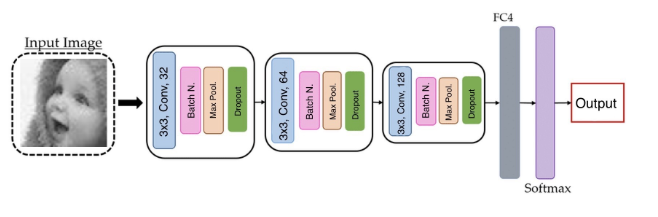
\includegraphics[width=\columnwidth]{Figures/CustomArch.png}
        \caption{Özay Ezerceli's~\cite{ezerceli_convolutional_2022} Proposed CNN Architecture}
        \label{fig:ozayCNNArchitecture}
      \end{figure}
      
      During the pre-processing phase of the dataset, preparation consisted of image resizing, denoising and rotation correction. This technique increased the input quality the model will process, learn from, and test. Ezerceli's~\cite{ezerceli_convolutional_2022} CNN model uses an input layer, twelve hidden layers and a connected output layer. The hidden layers involve three blocks, using the template block of a 2D Convolutional with a batch number, Max Pooling and a Dropout layer. Using the template block mentioned is repeated three times with a batch number starting at 32 and doubled each time. The last step in classifying involves an output layer with a Fully Connected Softmax activation layer.

      Three architectures discussed by Manali Shaha~\cite{shaha_transfer_2018} in the research paper, `Transfer learning for image classification' experiments three architectures with two `state-of-the-art' databases named GHIM10K and CalTech256, `AlexNet', `VGG-16', and `VGG-19'. Shaha~\cite{shaha_transfer_2018} rates the VGG-19 architecture, quoting `Improved VGG16 architecture overcomes the drawbacks of AlexNet and increases the system accuracy.', indicating that the AlexNet has drawbacks, and VGG-16 is significantly better than AlexNet. VGG-19 achieves a better recall, precision and F-score than VGG-16 and AlexNet. 

      \begin{figure}[htp]
        \centering
        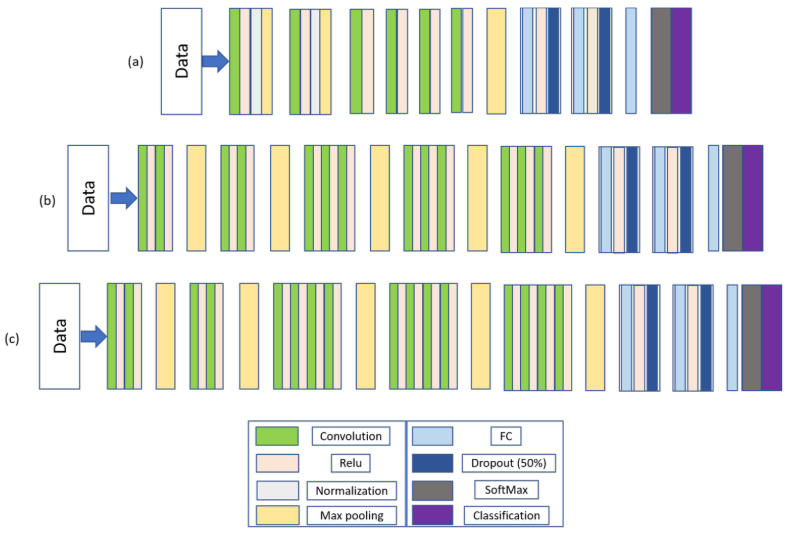
\includegraphics[width=\columnwidth]{Figures/Architectures.png}
        \caption{Manali Shaha's~\cite{shaha_transfer_2018} Architecture Illustrations of AlexNet~\cite{krizhevsky_imagenet_2012}, VGG-16~\cite{simonyan_very_2015} and VGG-19~\cite{simonyan_very_2015}}
        \label{fig:shahasIllustrationCNNArchitectures}
      \end{figure}
      
      A Journal Article written by Gede Putra Kusuma~\cite{kusuma_emotion_2020} mentions a VGG-16; refer to the illustration by Shaha~\cite{shaha_transfer_2018},~\ref{fig:shahasIllustrationCNNArchitectures} and Global Average Pooling (GAP); allowing the CNN to overcome overfitting and underfitting.~\cite{lin_network_2014}. The researchers chose VGG-16 out of VGG-19 as the infrastructure is too complex for the researcher's Use Case. Kusuma notes, `both architecture demonstrated similar results as reported in~\cite{simonyan_very_2015}.' The VGG-16 and GAP model achieves 69.40\% within this paper for the FER-2013 dataset. The article mentioned three suggested optimisers: ' Stochastic Gradient Descent (SGD)', `Adam' and `SWATS'. The author~\cite{kusuma_emotion_2020} continues with `An alternative to SGD was proposed in~\cite{kingma_adam_2015} and coined as Adam to overcome SGD's limitation.'

      Furthermore, Shallu Sharma~\cite{shaha_transfer_2018} experiments with optimisers using CNN for multi-classification. The researcher chooses a learning rate of `0.0001' for Adam, AdaGrad and Gradient Descent. However, the learning rate `0.001' was given to the RMSProp. The Adam optimiser with the Cross-entropy loss function was the best performer, achieving an 83.67\%. The second and third top performers were RMSProp, and Gradient Descent, being 76.9\% and 69.40\%. The research compares pooling strategies, showing that Adam and Max-Pooling achieve 83.67\% and Average Pooling achieves 66.10\%. These statistics may indicate that the Adam optimiser may perform better with architectures that use Max-Pooling layers.

      Focusing on performance, as the VGG-16 and VGG-19 seem to be heavily structured, training models could be slow and time-consuming, especially if the model was stored in runtime, as any data loss would result in rebuilding and training the model. Faten Khemakhem~\cite{khemakhem_facial_2019} suggests using a GPU to build and train the architecture. The hardware used to build and train the model was an Intel Core i7 CPU and an NVIDIA GeForce G920MX GPU. The paper suggests, `Thus learning times can be reduced with GPU cores compared to a CPU. Although GPU cores are slower than CPU cores, they largely offset this disadvantage by their large numbe and faster memory.'~\cite{khemakhem_facial_2019}

    \section{Methodology}
      \subsection{Objectives}
        The main objectives of this project are to develop an accurate FER model using CNNs and to improve the model's performance on specific tasks. The following steps be undertaken to achieve these objectives:-

        \begin{enumerate}
          \item Dataset Preparation: Mapping the train and test emotions and images using folder names and file paths to achieve this. A Python snippet helps with the Dataset Preparation phase.
          \item Pre-processing: Read in the mapping datasets and extract the emotion and file paths. The file paths allow the images to open within the Python script. The pre-processing will apply data augmentation techniques to increase the number of images lacking within the `disgust' train and test class.
          \item Architecture Selection and Optimisation: Investigate different CNN architectures, considering the arrangement and design of layers and connections of the architecture. Analysing any previous research on FER builds an understanding and identifies any potential issues and optimisations that can enhance the model's accuracy and performance. OpenCV or Kera's Image Pre-Processing tools benefit in this phase to improve the experiment's training, validation and testing phases.
          \item Evaluation Techniques: A few methods to analyse and evaluate the model's performance and accuracy regarding the learning and predictive classifications. Classification Reports and Confusion Matrices to identify optimisation issues to improve accuracy results. Training and validation evaluation methods are required to determine the model's learning quality. The Tensorflow provides a Pandas DataFrame of history when a model is fitted, which includes `loss' and `val\_loss' to determine the optimisation of the learning state of the model. An evaluation of validation data is essential, too, to highlight any errors within the preparation phase.
        \end{enumerate}

      \subsection{Pre-Processing}
        The train and test images and emotions need to be mapped. A decent method is creating a Python snippet to read through the dataset of both train and test directories and record the emotions from the parent directory name and file path to the files within. The dataset requires some work before any pre-processing can happen. During this process, a condition to control what classes to include in the mapping data, as the experiment involves four classes.

        The pre-processing phase will read the rows of the mapping data, record the emotion and open the image with the file-path column to start the pre-processing process. The pre-processing stage focuses on randomising the mapping data and any necessary augmentations. OpenCV or Kera's Image Pre-Processing tools benefit in this phase to improve the experiment's training, validation and testing phases.

        Data augmentation is necessary for the experiment with the lack of train and test data for the emotion of disgust. This technique means that in the testing of the dataset, the classifier would avoid the disgust emotion as there is not enough training, validation or even test data to give the model a chance to identify patterns. The pre-processing scripts would flatten the data and store it into train and test datasets with label and pixel columns. All datasets will have a rescale of $\frac{1}{255}$ using ImageDataGenerator's flow to normalise the data from 0 to 1. The emotion, disgust, will have additional treatment, including `rotation\_range = 20', `zoom\_range=0.15', `width\_shift\_range=0.2', `height\_shift\_range' and `fill\_mode = "nearest"' that would repeat seven times each, resulting in 3052 train images and 777 test images.

      \subsection{Architecture}
        Architecture is the arrangement and design of layers with the understanding of different connections within the network. Different architectures change the flow of CNN and may not always perform well for various image classification tasks compared to others. These can be down to the underlying issues with the methods used within the model architecture, where other model architecture is overcome. The prior research of both architectures in general and FER-2013-specific experiments using different architectures helps picture potential issues with architectures and form an understanding of possible integrations with the architectures to optimise accuracy and performance.

        The VGG-19 architecture is favourable for the FER-2013. The model is effective regarding image classification tasks, including FER. As the architecture's name suggests, the model consists of nineteen layers and requires significant computational resources for training and testing. Thus, a configuration of OS: Debian 11, Driver: ROCm, Library: Tensorflow 2, CPU: Ryzen 7 3700X, AMD Radeon 5700XT and 32GB (4x8GB | 4x3200MHz) RAM, which would optimise the learning and testing of the model. This model is possible with the available sources that come along with the tasks for the experiment setup.

        VGG-19 architecture~\ref{fig:shahasIllustrationCNNArchitectures} consists of the input layer, sixteen Convolutional layers, a max pooling layer after each set of Convolutional layers, three fully connected layers with 4096 units, and a Softmax. An input layer takes in the raw image and applies some initial processing, such as resizing the image to a fixed size. The Convolutional layers apply a filter to the images; the set of layers starts from 64 and goes up to 512 filters. Max Pooling layers reduce the spatial size of the feature maps. Fully Connected layers process the flattened feature maps from the last Convolutional layer and output a feature vector for classification. Softmax is used to produce a probability distribution over the possible classes. 

        In summary, the architecture contains sixteen Convolutional with Max Pooling layers after each set of Convolutional layers, three Fully Connected and Softmax layers. It is also worth noting that the first thirteen Convolutional layers use 3x3 filters, whilst the last three use 1x1 filters.

        ELU is a refined version of the ReLU, adding smoothness, so the expected results should improve the model's performance. The ELU activation is proposed to test the difference between the model. This activation will put the model to the test and understand the differences.

      \subsection{Optimisers}
        In Machine Learning, optimisation refers to finding the parameters of a model that minimises a loss function. A loss function measures the model's performance when learning using classification or regression methods. 
          
        After some in-depth research, `SGD', `Adam', and `SWATS' were explored, and Gede Putra Kusuma~\cite{kusuma_emotion_2020} suggested that Adam overcomes SGD's limitations. On top of that, Shallu Sharma~\cite{sharma_optimised_2021} proceeds to experiment with `Adam', `AdaGrad', `Gradient Descent' and `RMSProp' optimisers and found that Adam optimiser was not only a high achiever, but works well with Max-Pooling, which the VGG-19 architecture is based on. The learning rate chosen is `0.0001' for the recommendation from Sharma~\cite{sharma_optimised_2021}.

    \section{Results}
      \subsection{VGG-19 Architecture | Activation: ReLU}
        \begin{figure}[h]
          \centering
          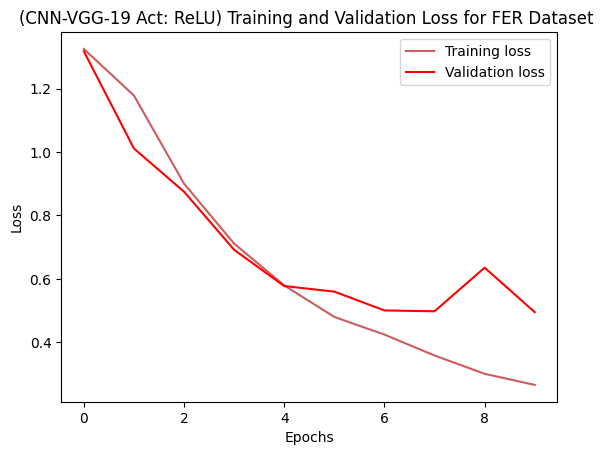
\includegraphics[width=\columnwidth]{Figures/FER-2013_VGG19-ReLU_TVL.png}
          \caption{CNN: Validation and Training Loss for `VGG-19 Architecture | Activation: ReLU' model}
          \label{fig:cnnVGG19ReLUTVL}
        \end{figure}

        \begin{table}[h]
          \caption{CNN: Classification Report for the `VGG-19 Architecture | Activation: ReLU' model}
          \label{tab:cnnVGG19ReLUClassificationReport}
          \begin{tabular}{ccccc} 
            \hline
      
            \textbf{Class} & \textbf{Precision} & \textbf{Recall} & \textbf{F1-Score} & \textbf{Support} \\ 
            \hline
            Angry & 0.68 & 0.72 & 0.70 & 958 \\
            Disgust & 0.91 & 0.88 & 0.90 & 1332 \\
            Happy & 0.85 & 0.87 & 0.86 & 1774 \\
            Surprise & 0.84 & 0.79 & 0.81 & 831 \\ \hline
            Accuracy & & & 0.83 & 4895 \\ \hline
            Macro Avg. & 0.82 & 0.82 & 0.82 & 4895 \\ \hline
            Weighted Avg. & 0.83 & 0.83 & 0.83 & 4895 \\ \hline
            \multicolumn{5}{l}{\textbf{Accuracy Score}: 83\%}
          \end{tabular}
        \end{table}

        \begin{figure}[h]
          \centering
          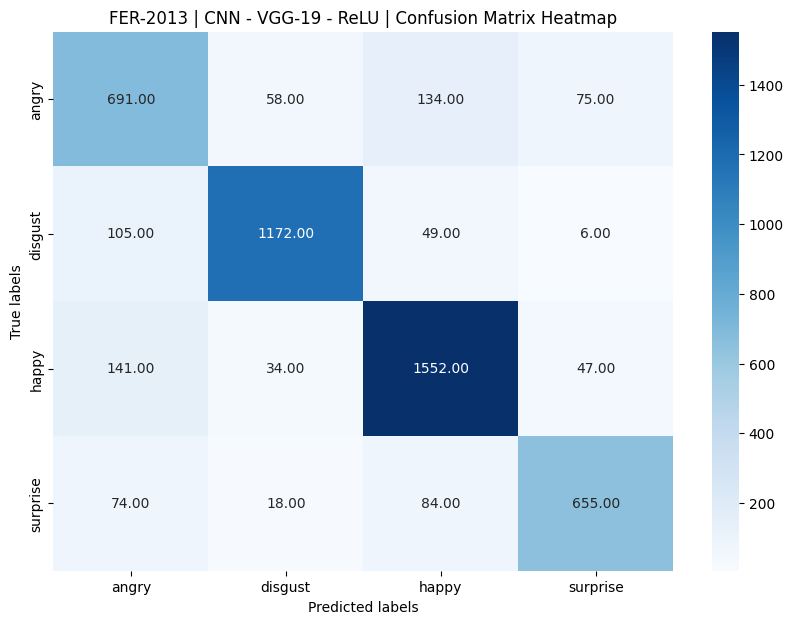
\includegraphics[width=\columnwidth]{Figures/FER-2013_VGG19-ReLU_CM.png}
          \caption{CNN: Confusion Matrix for `VGG-19 Architecture | Activation: ReLU' model}
          \label{fig:cnnVGG19ReLUConfusionMatrix}
        \end{figure}

      \subsection{VGG-19 Architecture | Activation: ELU}
        \begin{figure}[h]
          \centering
          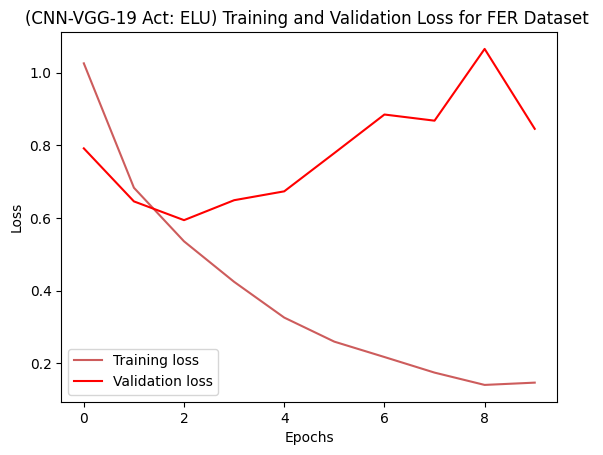
\includegraphics[width=\columnwidth]{Figures/FER-2013_VGG19-ELU_TVL.png}
          \caption{CNN: Validation and Training Loss for `VGG-19 Architecture | Activation: ELU' model}
          \label{fig:cnnVGG19ELUTVL}
        \end{figure}

        \begin{table}[h]
          \caption{CNN: Classification Report for `VGG-19 Architecture | Activation: ELU' model}
          \label{tab:cnnVGG19ELUClasificationReport}
          \begin{tabular}{ccccc}
            \hline
            \textbf{Class} & \textbf{Precision} & \textbf{Recall} & \textbf{F1-Score} & \textbf{Support} \\
            \hline
            Angry & 0.65 & 0.66 & 0.66 & 958 \\
            Disgust & 0.92 & 0.87 & 0.89 & 1332 \\
            Happy & 0.82 & 0.82 & 0.82 & 1774 \\
            Surprise & 0.73 & 0.79 & 0.76 & 831 \\ \hline
            Accuracy & & & 0.80 & 4895 \\ \hline
            Macro Avg. & 0.78 & 0.79 & 0.78 & 4895 \\ \hline
            Weighted Avg. & 0.80 & 0.80 & 0.80 & 4895 \\ \hline
            \multicolumn{5}{l}{\textbf{Accuracy Score}: 80\%}
          \end{tabular}       
        \end{table}
        \begin{figure}[h]
          \centering
          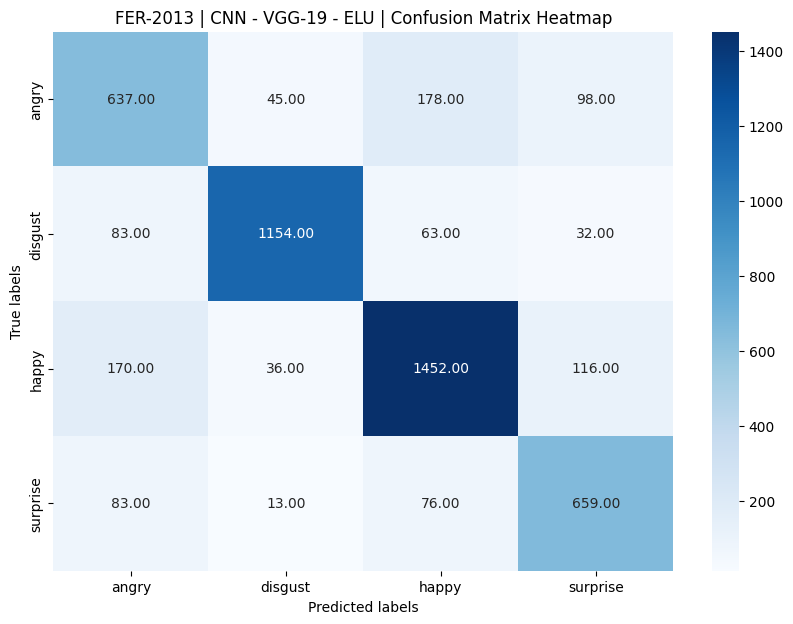
\includegraphics[width=\columnwidth]{Figures/FER-2013_VGG19-ELU_CM.png}
          \caption{CNN: Confusion Matrix for `VGG-19 Architecture | Activation: ELU' model}
          \label{fig:cnnVGG19ELUConfusionMatrix}
        \end{figure}

    \section{Discussion}
      Figures (\ref{fig:cnnVGG19ReLUTVL},~\ref{fig:cnnVGG19ELUTVL}) display the training and validation loss of the model's learning curve. The VGG-19, with the activation of ELU, show that the validation of the model starts to gap the training aspect with a significantly more significant loss of 0.3 and then proceeds to overfit with a massive gap of up to 1.20 from 0.2 by the eighth epoch. The original VGG-19 architecture starts with a decent curve and has a validation loss following the training loss. It shows a lack of overfitting and underfitting during the learning process. However, the validation loss loses track with the training loss by the fourth epoch and has a loss of 0.3, between 0.4 and 0.7 by the eighth epoch. The training accuracy of VGG-19 architecture achieves 90.73\%, and the validation accuracy reaches 83.31\%. VGG-19 customised architecture with ELU achieves a training accuracy of 95.17\%, and the validation accuracy achieves 77.59\%. Jinu Lilly Joseph~\cite{joseph_facial_2021} performs 67.18\% on training using 150 epochs; this difference is 23.55. The accuracy may be lower because, in this experiment's class selection, disgust only has four hundred and thirty-six train one hundred and eleven test images, duplicated and pre-processed with the methods discussed in the methodology section. This result could indicate that Jinu's~\cite{joseph_facial_2021} selection has natural facial emotions on both train and test images, meaning a lower overall percentage.

      Although the VGG-19 architecture requires computational power, the model achieves an overall 83\% testing accuracy, which is a significant accuracy. In contrast, the model with ELU activation performs a general of 80\%. Jinu Lilly Joseph~\cite{joseph_facial_2021} conducts a similar experiment with a custom CNN architecture, testing `neutral', `happy', `angry' and `fear', training with forty epochs, with the early stopping of the model fit. The researcher achieves a 75.55\% testing of the model with the cleansed version of the dataset. The experiment achieves a 7.45\% difference compared to Jinu's~\cite{joseph_facial_2021} experiment. This accuracy could be down to the VGG-19 architecture, class selection and pre-processing techniques used, as our experiment uses `disgust' and `surprise' emotions compared to `neutral' and `fear'. 
      Tables (\ref{tab:cnnVGG19ReLUClassificationReport},~\ref{tab:cnnVGG19ELUClasificationReport}) demonstrate the model's testing Classification Report. The statistical data shown in the report indicates the class's performance and helps evaluate the model's performance, errors and accuracy. Angry precision is 68\%, with activation of ReLU and 65\% with activation of ELU. This observation shows that the ReLU activation has a higher precision than three per cent. The recall is much higher with the ReLU activation than the ELU activation, and the F1-score of activation of ReLU is higher than the ELU activation. The ELU activation performs better within the precision, recall and F1-score for disgust than the ReLU activation.

      Figures (\ref{fig:cnnVGG19ReLUConfusionMatrix},~\ref{fig:cnnVGG19ELUConfusionMatrix}) visualises the Confusion Matrices. This evaluation tool represents the support of each emotion and demonstrates any true and false positives of the model's performance. The Confusion Matrices of VGG-19 with ReLU and ELU activation have a similar fitting. However, the VGG-19 with ReLU activation has a better fitting overall. The disgust emotion had zero true and false positives when the training was left at the original number of train and test images. The pre-processing fixed this issue.

    \section{Conclusion}
      In conclusion, the standard VGG-19 architecture performed better than the ELU activation parameter. The VGG-19 performed better, as suggested by Manali Shaha~\cite{shaha_transfer_2018}. The optimisation and learning rate presented by Shallu Sharma~\cite{sharma_optimised_2021} improved the performance and accuracy of the model from the Validation and Training Loss. The learning rate for the VGG-19 model with the Adam optimiser and Cross-Entropy loss function shows that the learning aspect of the model falls into a curve. This visualisation indicates that the loss of validation and training is too steep and that the model seems to learn effectively. The VGG-19 model achieves 90.73\% training and 83.31\% validation accuracy for the learning aspect. The customised VGG-19 model conducts training of 95.17\% and 77.59\% validation accuracy. The testing of the model with ReLU activation of 83\% accuracy and 80\% for the model with the ELU activation shows a 3\% difference.

    \section{Terminology}
      List of terminologies used in this document:-
      \begin{itemize}
        \item FER-2013 - Facial Expression Recognition.
        \item CNN - Convolutional Neural Network.
        \item SGD - Stochastic Gradient Descent.
      \end{itemize}
    
  %\nocite{*}
	\renewcommand\refname{\section{Reference List}}
	\small{\bibliographystyle{IEEEtran}
    \bibliography{ref}}
\end{document}